\documentclass[12pt,a4paper]{report}

\usepackage[utf8x]{inputenc}
\usepackage{amsmath}
\usepackage{amsfonts}
\usepackage{amssymb}
\usepackage{graphicx}
\usepackage{enumitem}
\usepackage{pgf}
\usepackage{tikz}
\usepackage{calrsfs}
\usepackage{algpseudocode}
\usetikzlibrary{arrows,automata,calc, positioning}

\begin{document}

\begin{titlepage}
	\centering
	{\scshape\LARGE Universidad Nacional Autónoma de México \par}
	\vspace{1cm}
	{\scshape\Large Computación Distribuida\par}
	\vspace{1.5cm}
	{\huge\bfseries Tarea 3\par}
	\vspace{.5cm}
	{\Large\itshape Edgar Quiroz Castañeda \par}
    \vspace{.5cm}
	{\Large\itshape Jerónimo Almeida Rodríguez \par}
	\vfill
	 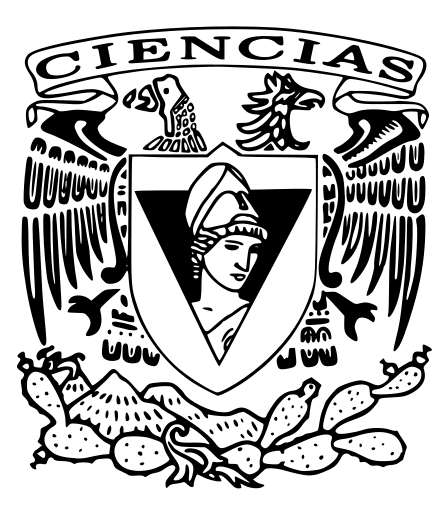
\includegraphics[width=0.5\textwidth]{escudo_f-ciencias.png}
	\vfill

% Bottom of the page
	{\large Jueves 30 de Agosto del 2018 \par}
\end{titlepage}

\pagebreak
\setlength{\voffset}{-0.75in}
\setlength{\headsep}{5pt}

\newcommand{\ed}[2]{(#1) edge (#2)}
\newcommand{\eee}[4]{\path [->,draw,thin] ($ (#1) !.5! (#2)$) -- ($ (#3) !.5! (#4) $);}


\begin{enumerate}
		%Ejercicio 1
		\item {
		Dados los procesos $A$ y $B$, diseña un algoritmo para el ataque coordinado
		proximado(aproximate agreement) en el que para llegar al acuerdo deben decidir
		valores que estén a distancia a lo más $\frac{1}{2^k}$ y utilice menos rondas
		de comunicación que el algoritmo visto en clase.
	}
	\item {
		Dibuja la gráfica del protocolo que diseñaste para 2 rondas para $k = 2$.
		Para cada vértice indica el valor de salida y para cada arista indica el
		patrón de mensajes recibidos.
	}
\end{enumerate}
\end{document}
